
\title[Code Reviews]{Code Reviews}
\date{}
\author[Pepe Doval]{}
\institute{}

\section{Code Reviews}
\label{sec:CodeReviews}

\usebackgroundtemplate{}
\begin{frame}
  \titlepage
\end{frame}

\usebackgroundtemplate{%
  \tikz[overlay,remember picture] 
  \node[opacity=0.3 , at=(current page.south east),anchor=south east] {
    
\includegraphics[]{logo-labs}};
}

\subsection{Introdución}
\label{subsec:Introducion}

\begin{frame}
  \frametitle{Canta xentiña!}
  \begin{figure}[ht]
    
\includegraphics[scale=0.18]{David_al_microfono}
  \end{figure}
\end{frame}

\begin{frame}
  \frametitle{Son un mal programador}
  \begin{figure}[ht]
    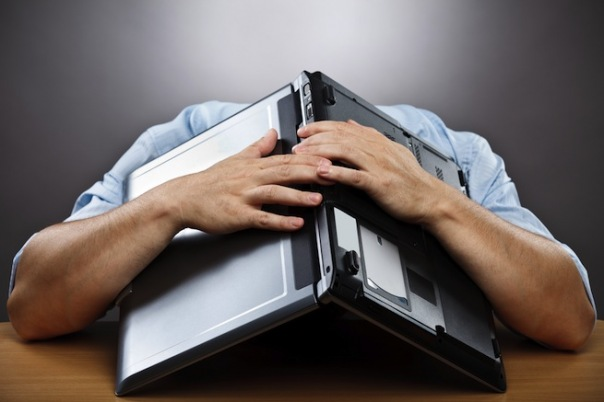
\includegraphics[scale=0.4]{sad_developer}
    \caption{http://csgardner.com/blog/2015/06/11/managing-software-developers/}
  \end{figure}
\end{frame}

\begin{frame}
  \frametitle{Pero tamén fun un crack}
  \begin{figure}[ht]
    
\includegraphics[scale=0.4]{zen_developer}
    \caption{https://www.apico.net/blog/how-bad-software-developer-are-you.html}
  \end{figure}
\end{frame}

\begin{frame}
  \frametitle{...é dicir, fun Junior}
  \begin{figure}[ht]
    
\includegraphics[scale=0.4]{happy_monkey}
    \caption{https://www.apico.net/blog/how-bad-software-developer-are-you.html}
  \end{figure}
\end{frame}

\begin{frame}
  \frametitle{De que vai construír software}
  \begin{figure}[ht]
    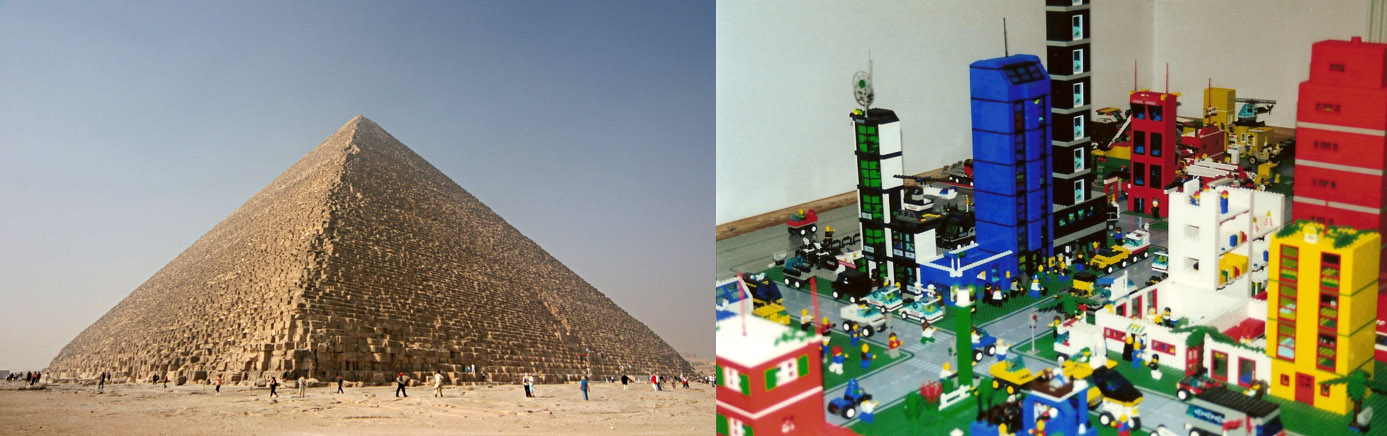
\includegraphics[scale=0.2]{pyramid_vs_lego}
    \caption{Wikipedia}
  \end{figure}
\end{frame}

\begin{frame}
  \frametitle{Abracemos o cambio}
    \centering
    O que hoxe está ben, mañá estará mal.
    \begin{figure}[ht]
      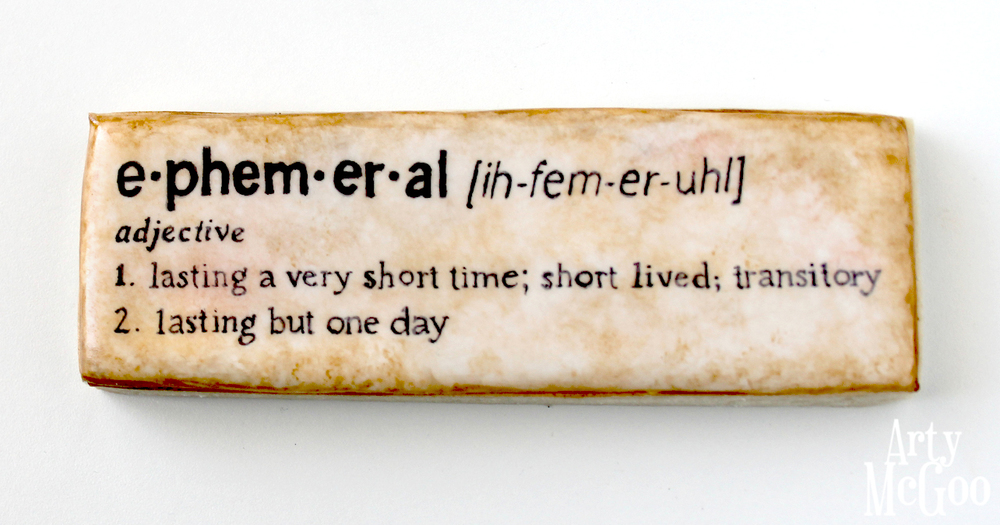
\includegraphics[scale=0.2]{ephemeral}
      \caption{http://www.artymcgoo.com/blog/2014/5/15/ephemeral-art}
    \end{figure}
\end{frame}

\begin{frame}
  \frametitle{Por que revisar código}
  \begin{itemize}
  \item Atopar erros
  \item Mellorar o código
  \item Compartir coñecemento
  \item Compartir decisións
  \item Mellorar a comunicación do equipo
  \end{itemize}
\end{frame}

\begin{frame}
  \frametitle{Mars Climate Orbiter}
  \begin{figure}[ht]
    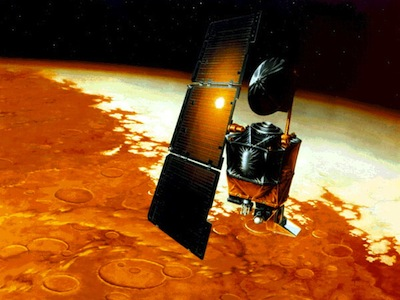
\includegraphics[scale=0.5]{mars_climate_orbiter}
    \caption{http://visionlearningcommunity.blogspot.com/2012/09/tragedies-in-science-crash-of-mars.html}
  \end{figure}
\end{frame}

\begin{frame}
  \frametitle{O día que non comezou a Terceira Guerra Mundial}
  \begin{figure}[ht]
    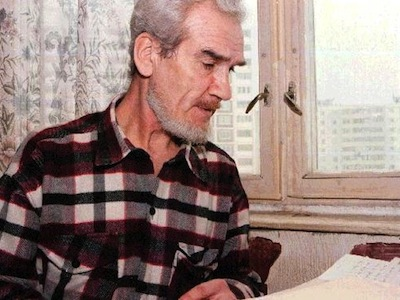
\includegraphics[scale=0.5]{petrov}
    \caption{http://www.brightstarsound.com/world\_hero/petrov\_expanded\_photo.html}
  \end{figure}
\end{frame}

\begin{frame}
  \frametitle{Se non queredes revisar código...}
  \begin{figure}[ht]
    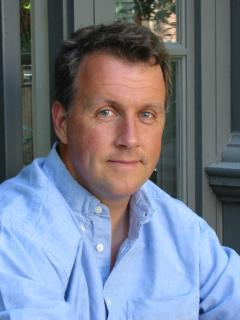
\includegraphics[scale=0.5]{Graham}
    \caption{Wikipedia}
  \end{figure}
\end{frame}

\subsection{Que é unha Code Review}
\label{subsec:Que}

\begin{frame}
  \frametitle{Que é unha Code Review}
  \begin{figure}[ht]
    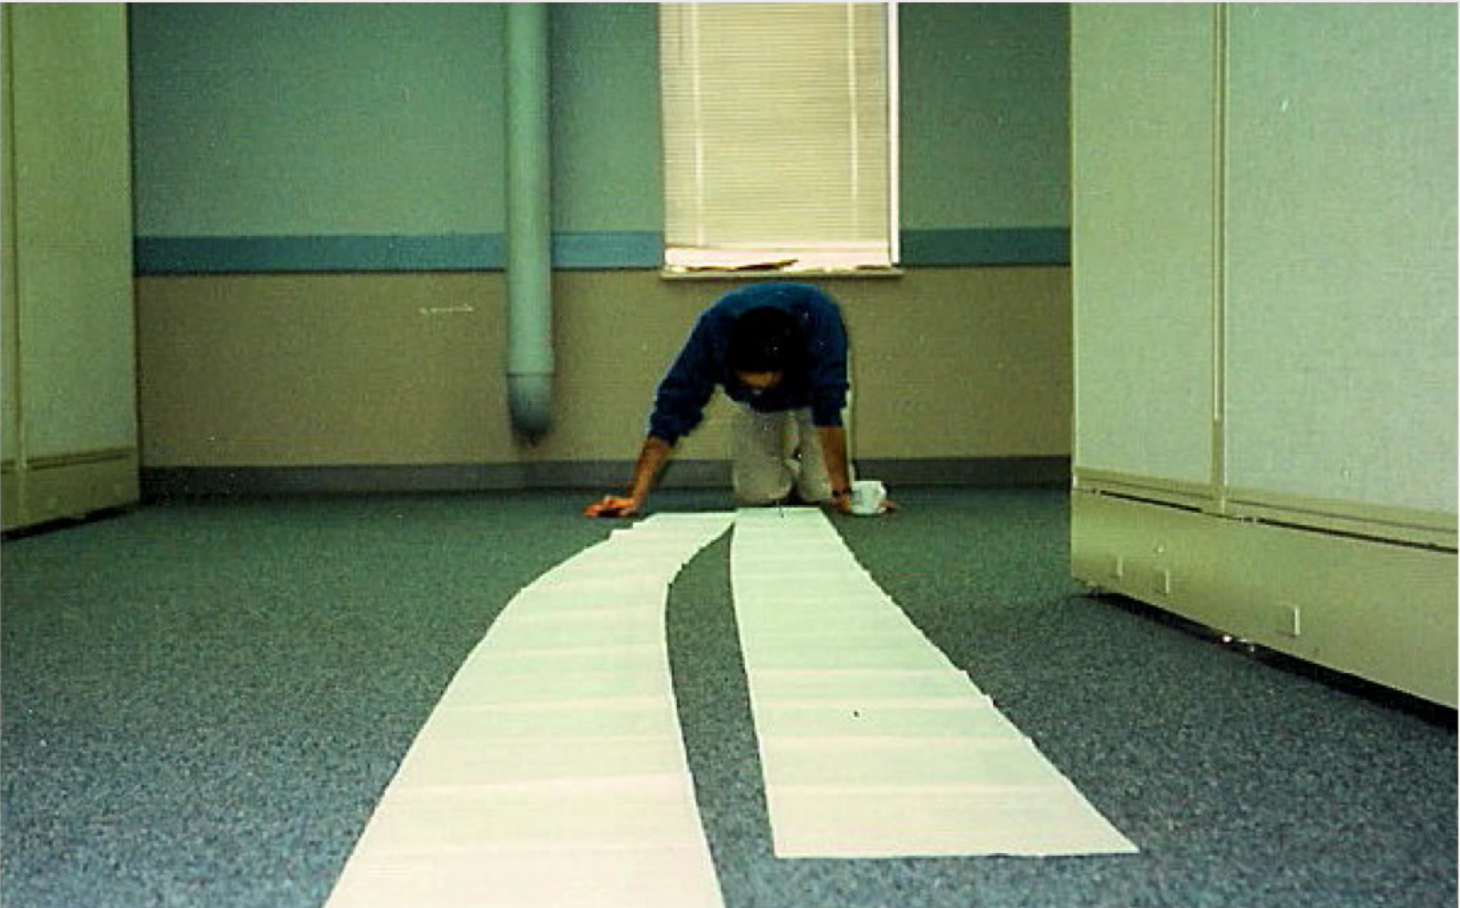
\includegraphics[scale=0.3]{old_code_review}
    \caption{https://www.youtube.com/watch?v=rHVlFOB5BpU}
  \end{figure}
\end{frame}

\begin{frame}
  \frametitle{Fases da Review}
  \begin{figure}[ht]
    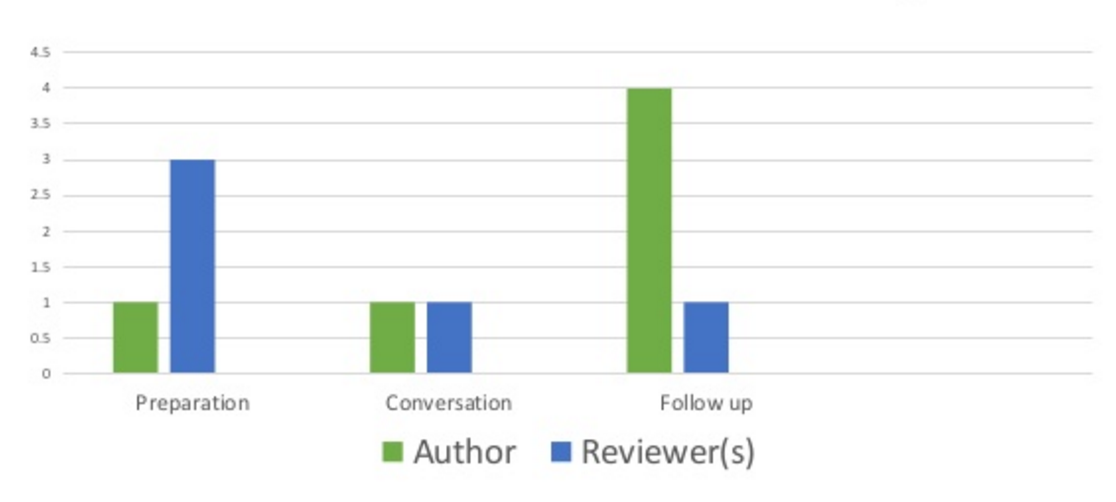
\includegraphics[scale=0.5]{not_a_meeting}
    \caption{http://www.slideshare.net/jprusakova/effective-codereview-color}
  \end{figure}
\end{frame}

\begin{frame}
  \frametitle{Limitade o tempo}
  \begin{figure}[ht]
    
\includegraphics[scale=0.3]{tired}
    \caption{https://sites.psu.edu/siowfa14/2014/10/19/why-am-i-so-tired/}
  \end{figure}
\end{frame}

\begin{frame}
  \frametitle{Facede unha checklist}
  \begin{figure}[ht]
    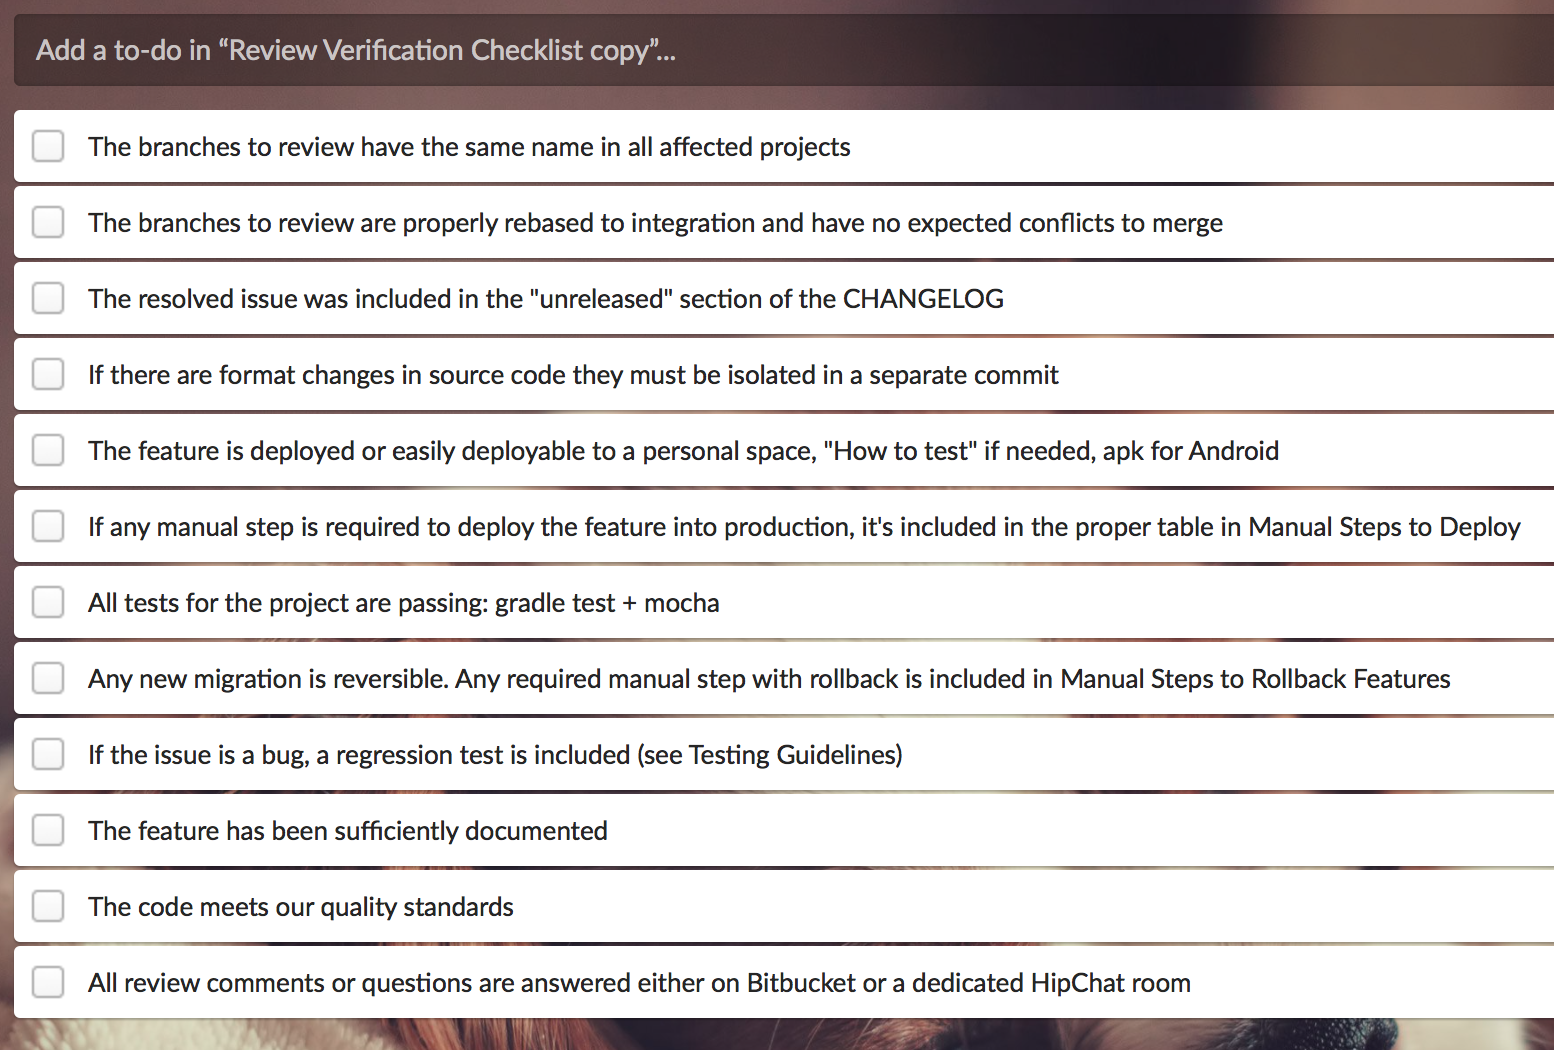
\includegraphics[scale=0.3]{review_checklist}
    \caption{My Review Checklist}
  \end{figure}
\end{frame}

\begin{frame}
  \frametitle{Medide}
  \begin{figure}[ht]
    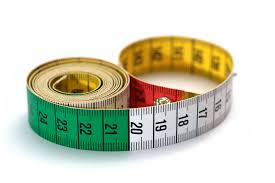
\includegraphics[scale=0.6]{metrics}
    \caption{Wikipedia}
  \end{figure}
\end{frame}

\begin{frame}
  \frametitle{Que midades!}
  \begin{figure}[ht]
    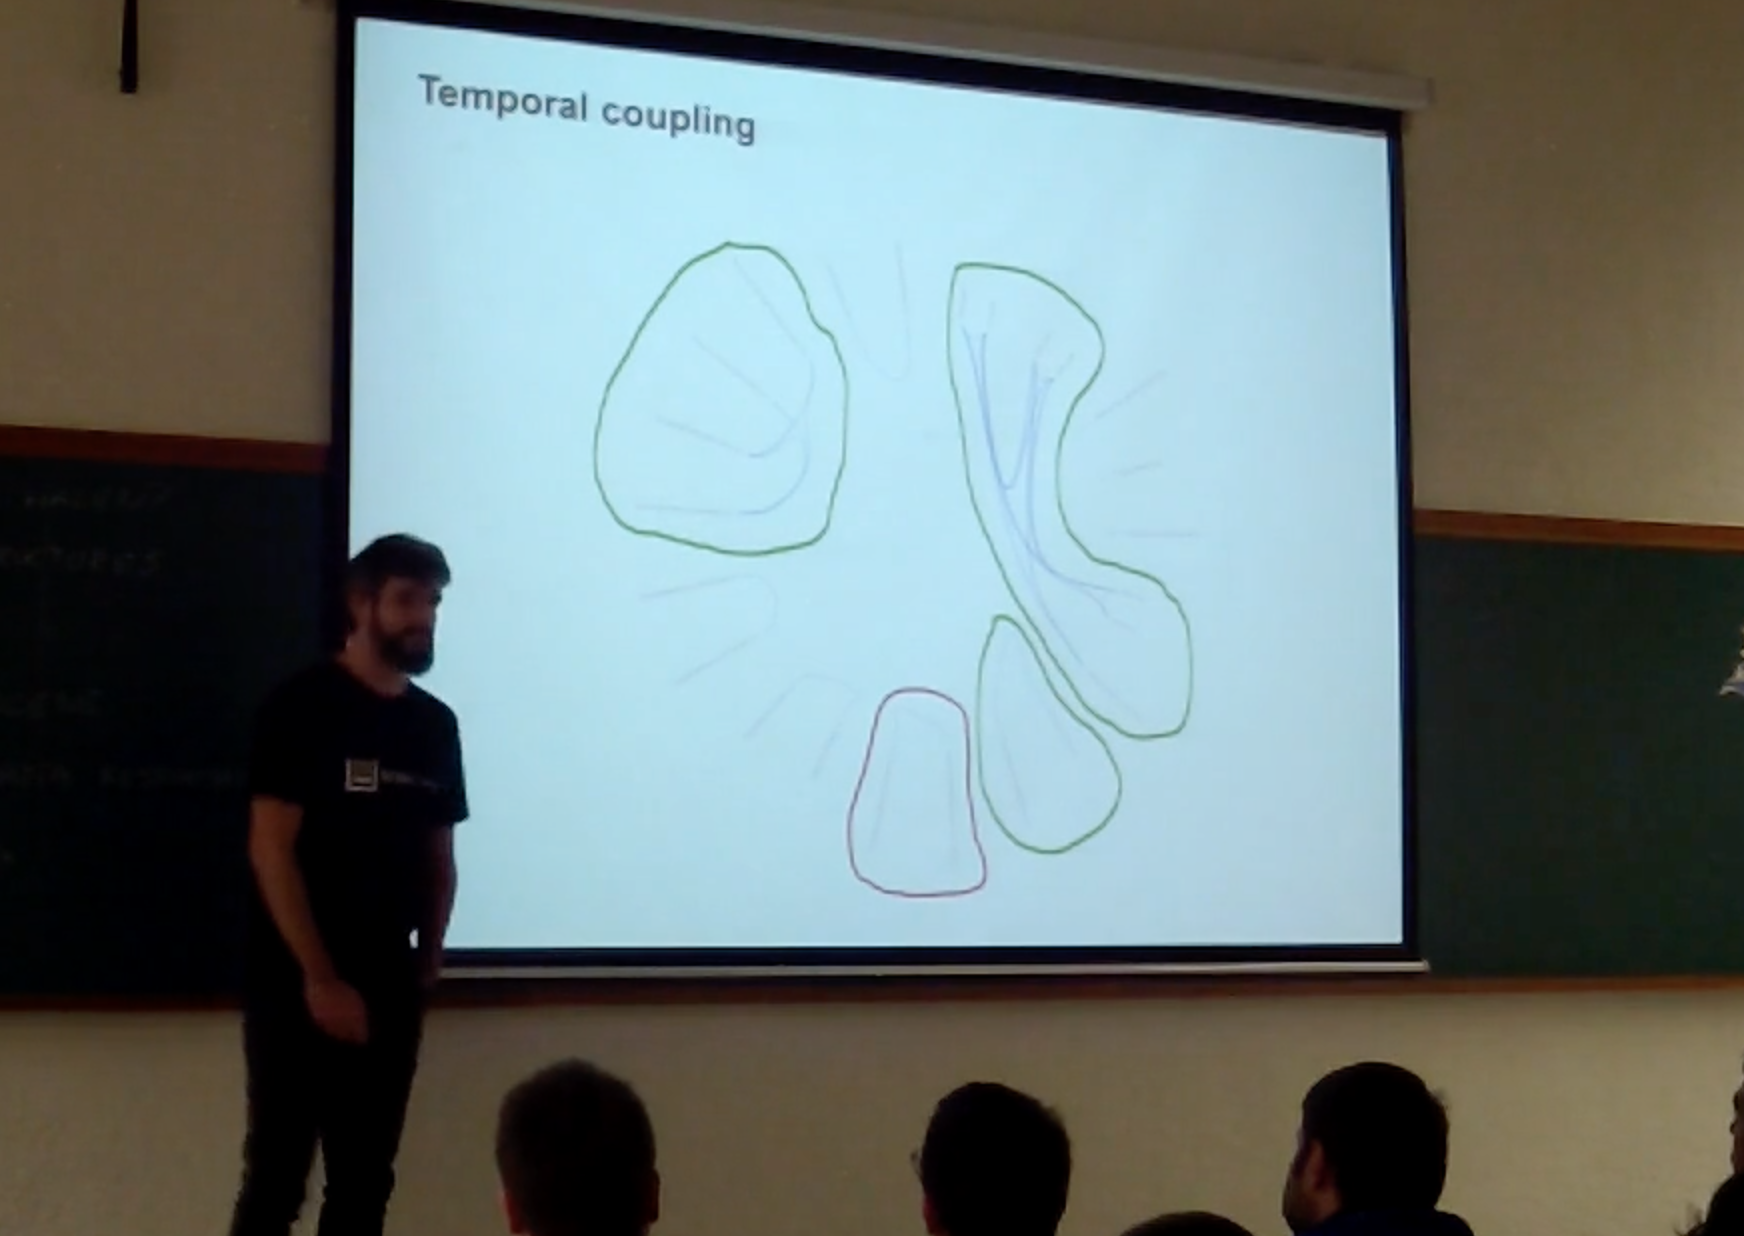
\includegraphics[scale=0.2]{vgaltes}
    \caption{Your Code as a Crime Scene - https://vimeo.com/154470784}
  \end{figure}
\end{frame}

\begin{frame}
  \frametitle{Medir é divertido, en serio}
  \begin{figure}[ht]
    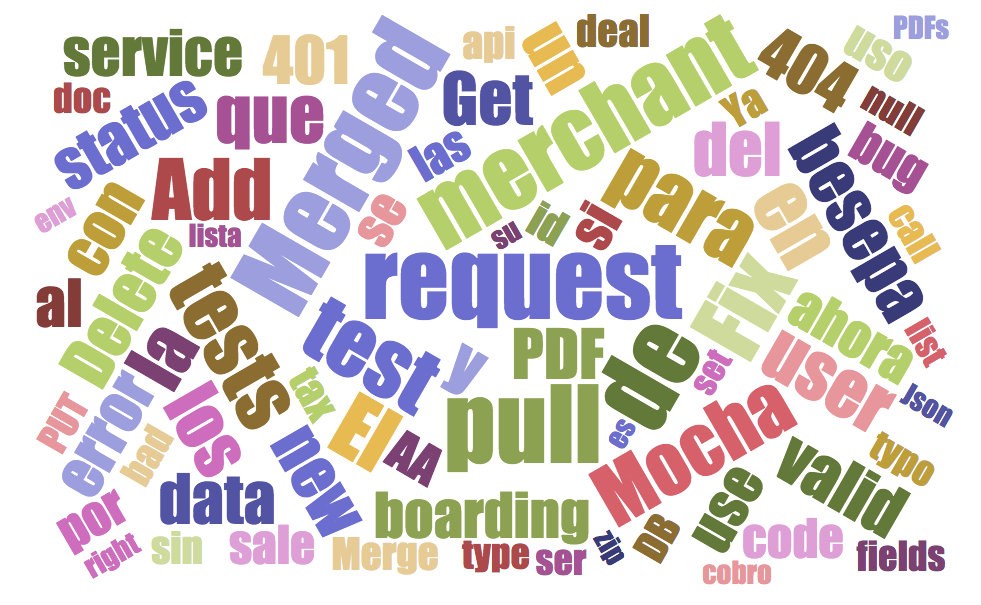
\includegraphics[scale=0.3]{tags}
  \end{figure}
\end{frame}

\begin{frame}
  \frametitle{Outra métrica sinxela}
  \begin{figure}[ht]
    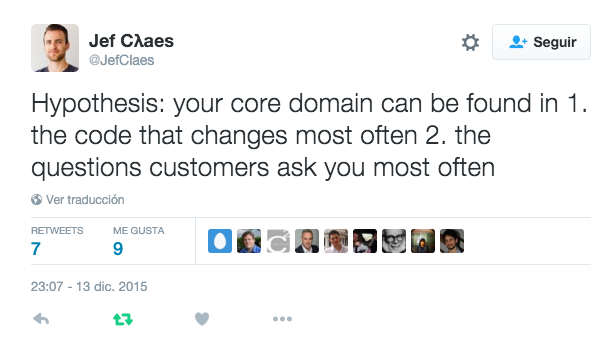
\includegraphics[scale=0.4]{your_domain}
  \end{figure}
\end{frame}

\begin{frame}
  \frametitle{Tips para reviewers}
  \begin{itemize}
    \item Limita o tempo
    \item Fai unha checklist
    \item Mide para decidir que abordar
  \end{itemize}
\end{frame}

\begin{frame}
  \frametitle{Fai pulls pequenas}
  \begin{figure}[ht]
    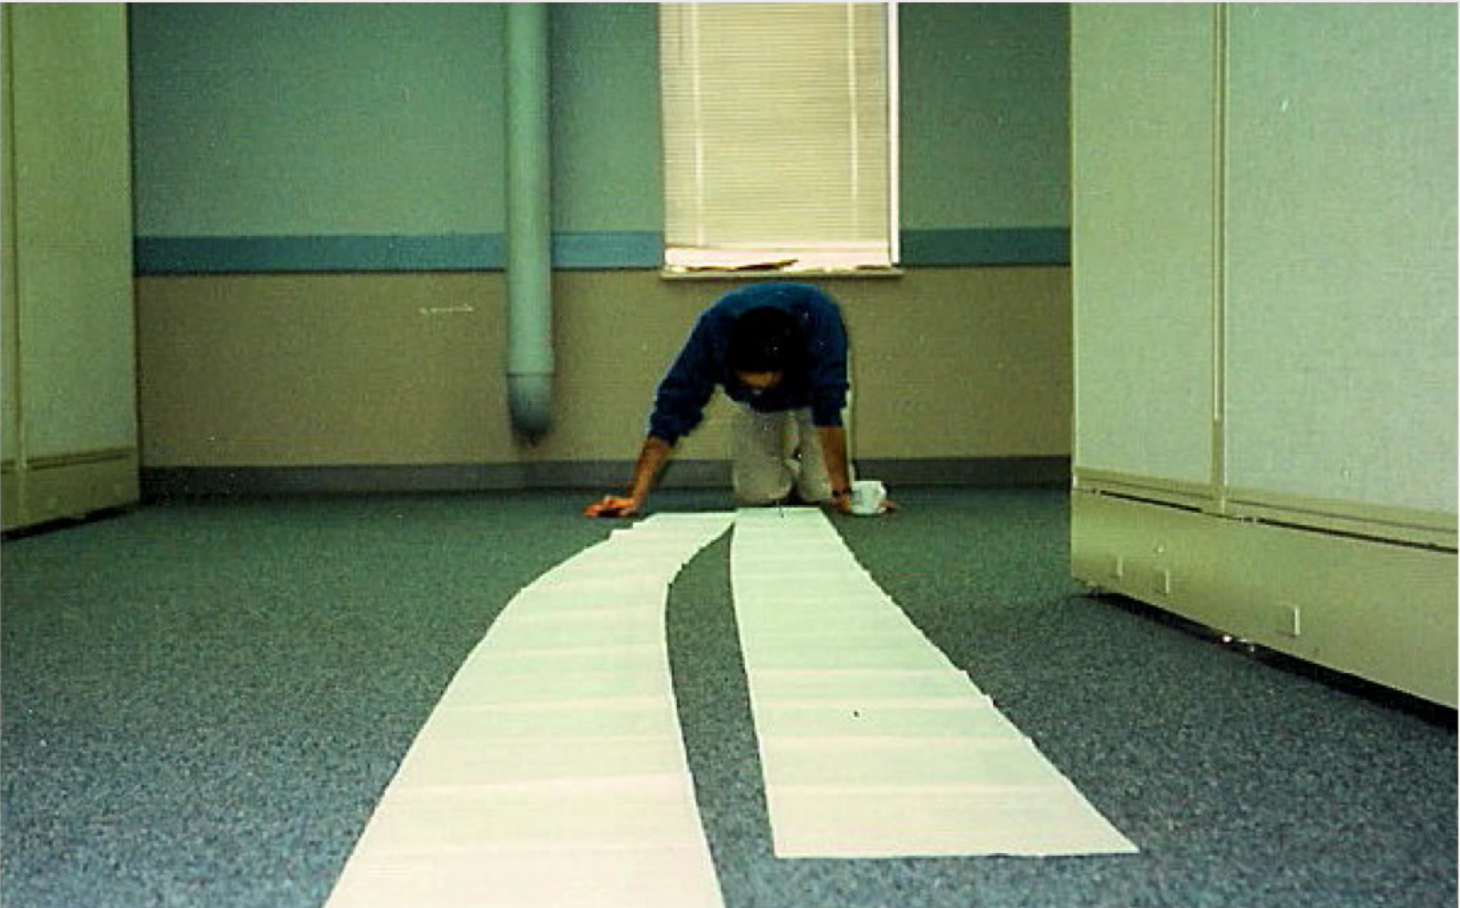
\includegraphics[scale=0.3]{old_code_review}
    \caption{https://www.youtube.com/watch?v=rHVlFOB5BpU}
  \end{figure}
\end{frame}

\begin{frame}
  \frametitle{Revisa ti antes}
  \begin{figure}[ht]
    \includegraphics[scale=0.2]{commit_push_run}
    \caption{https://www.reddit.com/r/ProgrammerHumor/comments/3nc531/in\_case\_of\_fire}
  \end{figure}
\end{frame}

\begin{frame}
  \frametitle{Automatiza}
  \begin{figure}[ht]
    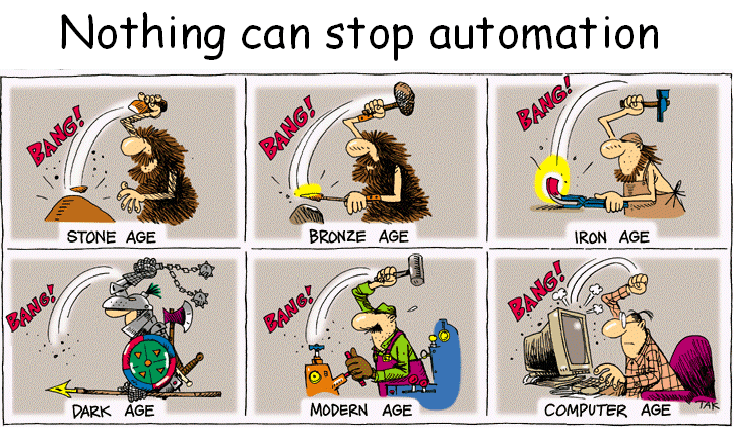
\includegraphics[scale=0.4]{automation}
    \caption{http://www.runmode.com/automationhumor.html}
  \end{figure}
\end{frame}

\begin{frame}
  \frametitle{Fai tests de regresión}
  \begin{figure}[ht]
    
\includegraphics[scale=0.3]{little_bugs}
    \caption{http://9gag.com/gag/a5dDw9o/99-little-bugs-in-the-code}
  \end{figure}
\end{frame}

\begin{frame}
  \frametitle{Tips para submitters}
  \begin{itemize}
    \item Fai pulls pequenas
    \item Revisa ti antes
    \item Automatiza
    \item Fai tests de regresión
  \end{itemize}
\end{frame}

\subsection{Como facer unha Code Review}
\label{subsec:Como}

\begin{frame}
  \frametitle{Big Brother vs Ego}
  \begin{figure}[ht]
    \centering
    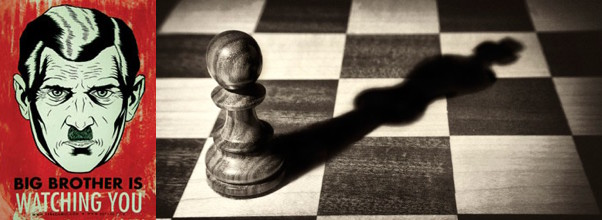
\includegraphics[scale=0.5]{ego}
    \caption{Wikipedia + http://www.sergerente.net/la-trampa-del-ego}
  \end{figure}
\end{frame}

\begin{frame}
  \frametitle{Acción vs visión}
  \blockquote{Vision without action is a dream. Action without vision is simply passing the time. Action with Vision is making a positive difference.}
  Joel Barker
\end{frame}

\begin{frame}
  \frametitle{Lei de Conway}
  \begin{figure}[ht]
    \centering
    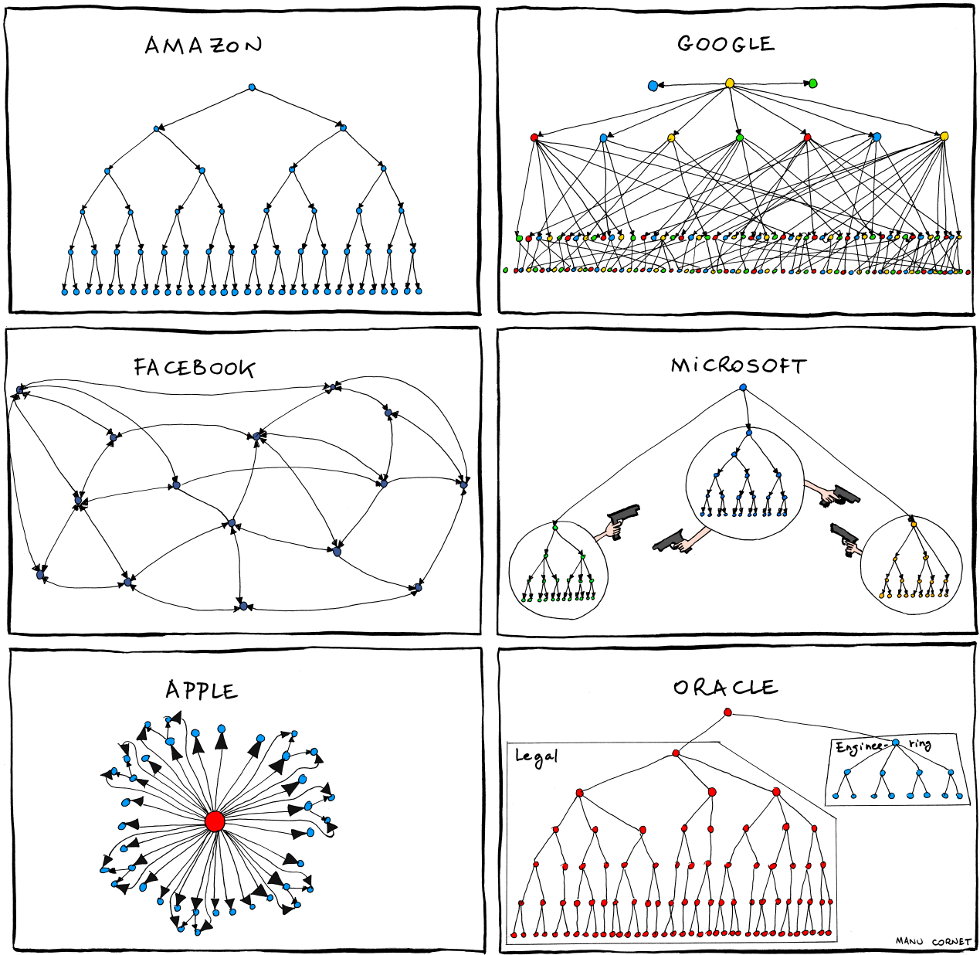
\includegraphics[scale=0.15]{conway}
    \caption{http://www.sixteensmallstones.org/conways-law-wiios-laws-software/}
  \end{figure}
\end{frame}

\begin{frame}
  \frametitle{Exceso de optimismo}
  \begin{figure}[ht]
    \centering
    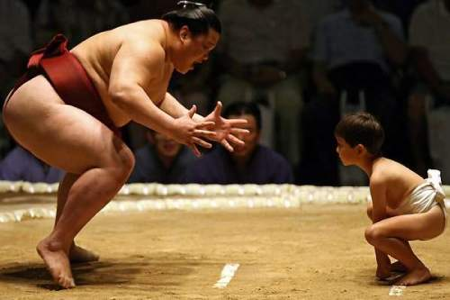
\includegraphics[scale=0.5]{optimism}
    \caption{https://mahifx.com/blog/aspects-of-behavioural-psychology-in-trading}
  \end{figure}
\end{frame}

\begin{frame}
  \frametitle{Lei de Parkinson da Trivialidade}
  \begin{figure}[ht]
    \centering
    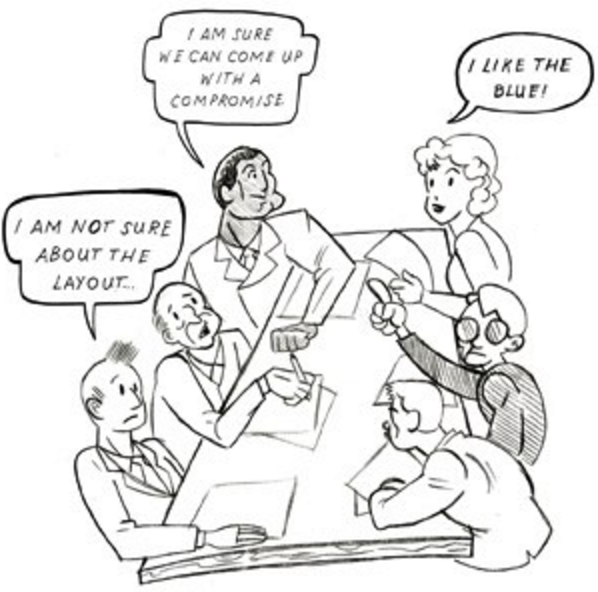
\includegraphics[scale=0.5]{triviality}
    \caption{http://www.zj86.cn/page/what-is-this\_net/fr/definition/triviality}
  \end{figure}
\end{frame}

\begin{frame}
  \frametitle{Tips}
  \begin{itemize}
    \item Chámase Code Review, non People Review
    \item Medide en vez de controlar
    \item Revisade todos
    \item Preguntade moito "por que"
    \item Discutide en persoa
    \item En lugar de ter razón, usade guías de estilo, métricas, ferramentas, ...
    \item Como submitter, ofrece contexto
    \item Como reviewer, pregunta alternativas
  \end{itemize}
\end{frame}

\begin{frame}
  \frametitle{Ideas para mellorar o código}
  \begin{itemize}
    \item Single Responsibility
    \item Open/Close
    \item Duplicación
    \item Eficiencia
    \item Manexo de erros
    \item Regra do boy scout
  \end{itemize}
\end{frame}

\begin{frame}
  \frametitle{Algúns malos olores}
  \begin{itemize}
    \item Nomes
    \item Lonxitudes
    \item Comentarios
    \item Número de parámetros
    \item Lexibilidade/estilo
  \end{itemize}
\end{frame}

\begin{frame}
  \frametitle{E o ingrediente segredo...}
  \begin{figure}[ht]
    \centering
    
\includegraphics[scale=0.15]{ingrediente_secreto}
    \caption{http://kungfupanda.wikia.com/}
  \end{figure}
\end{frame}
